\documentclass{llncs}
\usepackage{graphicx}

%\usepackage{graphicx}
%
\begin{document}

\title{ONJ Assignment - Predicting gender from Tweets \\
	\large PAN 2016 Author Profiling\\}


\author{Marko Novak Hindel, Jernej Ko{\v{z}}elj} 
\institute{Faculty of Computer and Information Science}
\maketitle

\begin{abstract}
Author profiling is the task of determining different attributes such as age, gender, native language or personality of an author. In our case we were focusing on determining just the gender. We took a Machine Learning approach to determine unknown author's gender based on plain text from tweets. We used SVM classifiers and were able to achieve an accuracy of 55.88\%.

\end{abstract}

\bigskip

\section{Introduction}\label{sec:Introduction}
Authorship analysis deals with the classification of texts into classes based on the stylistic choices of their authors. Beyond the author identification and author verification tasks where the style of individual authors is examined, author profiling distinguishes between classes of authors studying their sociolect aspect, that is, how language is shared by people. This helps in identifying profiling aspects such as gender, age, native language, or personality type. Author profiling is a problem of growing importance in applications in forensics, security, and marketing. E.g., from a forensic linguistics perspective one would like being able to know the linguistic profile of the author of a harassing text message (language used by a certain type of people) and identify certain characteristics (language as evidence). Similarly, from a marketing viewpoint, companies may be interested in knowing, on the basis of the analysis of blogs and online product reviews, the demographics of people that like or dislike their products. The focus is on author profiling in social media since we are mainly interested in everyday language and how it reflects basic social and personality processes\cite{PAN2016}.

\newpage

\section{Related work}\label{sec:Others}
This challenge is organized for the fourth time and each year there is something new added to author profiling task. For example one of really interesting related works is detecting the sentiment of text. You can train your model on corpus which consists of movie reviews and is accessible through nltk\cite{nltk} library. Sentiment analysis has been handled as a Natural Language Processing task at many levels of granularity. Starting from being a document level classification task, it has been handled at the sentence level and more recently at the phrase level. Microblog data like Twitter, on which users post real time reactions to and opinions about "everything", poses newer and different challenges. Some of the early results on sentiment analysis of Twitter data are Go et al. (2009), Bermingham amd Smeaton, (2010) and Pak and Paroubek (2010). Go et al use distant learning to acquire sentiment data. They use tweets ending in positive emoticonslike “:)” “:-)” as positive and negative emoticons like “:(” “:-(” as negative. They build models using Naive Bayes, MaxEnt and Support Vector Machines (SVM), and they report SVM outperforms other classifiers. In terms of feature space, they try a Unigram, Bigram model in conjunction of linguistic features like POS tags. They perform extensive feature analysis and feature selection and demonstrate that abstract linguistic analysis features contributes to the classifier accuracy.

\section{Methods}\label{sec:Others}



This problem associated with PAN 2016's task of author profiling involves the use of training data from a specific corpus given beforehand and evaluated on a different corpus. Profiling was done just in one dimension as mentioned in abstract - gender recognition. The training sets are available in English, Dutch and Spanish. We focused only on English language. As the corpus consists of XML files, we also got downloader which goes through all the files and populates it with actual text from tweets. There were some troubles getting all of the files because some of them were marked as null. We assumed that those were the deleted tweets, so we ignored them from our corpus. That don't mean they could affect end results by any means, because they were in minority, but we just got rid of them to work on proper and correct data.
Once we have our correct and useful data, we then divide it to training (90\%) and testing (10\%) set as we didn't get the formal testing set in corpus. So we improvised our own way.
For our features we check for the presence of hashtags, links and images. We also analyze punctuation; we use ratios of periods, question marks, exclamation marks and ellipsis’ compared to all the punctuation marks in a tweet. Then with all those features and classes we add them to scikit SVM, which trains the model. Then we feed SVM with testing data. Results are then compared to the truth file and that way we get accuracy. Our implementation is pretty basic, but we now know basic principles of text analysis using SVM which trains the model and then uses it on testing data.

\newpage

\noindent Support Vector Machine or (SVM) is a supervised machine learning algorithm which can be used for both classification or regression challenges. However,  it is mostly used in classification problems. In this algorithm, we plot each data item as a point in n-dimensional space (where n is number of features you have) with the value of each feature being the value of a particular coordinate. Then, we perform classification by finding the hyper-plane that differentiate the two classes very well. Support Vectors are simply the co-ordinates of individual observation. Support Vector Machine is a frontier which best segregates the two classes (hyper-plane/ line).

\bigskip
\bigskip

\begin{figure}[ht!]
\centering
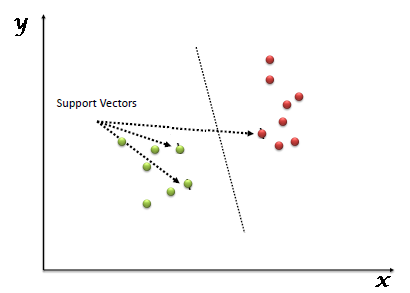
\includegraphics[width=120mm]{SVM_1.png}
\caption{Hyper-plane that differentiate different classes. \cite{SVMphoto}\label{overflow}}
\end{figure}

\newpage

\section{Evaluation and discussion}\label{sec:Others}
Since our work consisted of getting to know this method with SVM working, our results were not so bad. Our training takes about 15 to 20 minutes and testing another 10. We managed to get accuracy of determining the gender at about 55.88\% which is not that bad considering that our features from text were not so sophisticated. But as always there is room for improvements.


\bigskip
\section{Conclusion}\label{sec:Conclusion}

Our method and its results were comparable to those from the 2013 PAN challenge. The best thing is that we got closer to this kind of work and can now use it for many other interesting tasks in the future. Using SVM and other methods to get data or compare data. Future improvements would be to incorporate pronoun, determiner and preposition features as they are one of the most useful for gender recognition. Prepositions are markers of male writing, pronouns are markers for female writing. This is better explained in an article about automatically profiling the author of anonymous text by Shlomo Argamon from Illinois Institute of Technology\cite{Shlomo}.


\newpage

\begin{thebibliography}{1}

\bibitem{Einstein}
A. Einstein, On the movement of small particles suspended in stationary liquids required by the molecular-kinetic theory of heat, Annalen der Physik 17, pp. 549-560, 1905.


\bibitem{PAN2016}
Author Profiling, PAN 2016, http://pan.webis.de/clef16/pan16-web/author-profiling.html

\bibitem{SVMphoto}
SVM photo, SVM, https://www.analyticsvidhya.com/wp-content/uploads/2015/10/

\bibitem{Schlomo}
Automatically Profiling the Author of an Anonymous Text, http://u.cs.biu.ac.il/~koppel/papers/AuthorshipProfiling-cacm-final.pdf


\end{thebibliography}

\end{document}